%!TEX root = ../template.tex
%%%%%%%%%%%%%%%%%%%%%%%%%%%%%%%%%%%%%%%%%%%%%%%%%%%%%%%%%%%%%%%%%%%%
%% chapter2.tex
%% NOVA thesis document file
%%
%% Chapter with the template manual
%%%%%%%%%%%%%%%%%%%%%%%%%%%%%%%%%%%%%%%%%%%%%%%%%%%%%%%%%%%%%%%%%%%%

\typeout{NT FILE chapter2.tex}%

\chapter{Background}\label{cha:Background}

In this chapter we will discuss relevant work considering the goals of the work
to be conducted in this thesis. In particular, we will focus on the following topics:

In Section~\ref{sec:membership_protocols} we discuss the differences between
the different kinds of membership systems as well as some implementations.

In Section~\ref{sec:consensus} we will discuss some consensus protocols.

In Section~\ref{sec:blockchain} we will discuss some different types of
blockchain protocols.

\section{Membership Protocols}\label{sec:membership_protocols}

This section introduces membership protocols that have been considered to
be implemented as part of the work that will be developed. We selected these
memberships to study due to their wide differences in properties and their
popularity in usage.

\subsection{Membership}\label{sub:membership}

A protocol where each node knows every other node in the network might work well
for small networks, but it is not a scalable solution since each node would need
to have \textit{n - 1} communications channels open at all time, being n the
amount of nodes in the system, and each node needs to be following any and all
changes to the system. This is not feasible since the number of links between
nodes would rise quadratically and networks can easily reach thousands of
participants. In order to overcome the challenges that arise from large networks,
we usually use partial view membership protocols. In these protocols each node only knows
and maintains information about a small selection of nodes in the systems,
making it a more scalable strategy than a total view protocol, since
the number of connections tend to grow at a logarithmic rate instead.

When maintaining a partial view, protocols usually follow one of two strategies
when managing their memberships:

\begin{itemize}
  \item \textbf{Reactive:} Using this strategy, the partial view undergoes alteration solely
when there are changes in membership, typically occurring when a node joins or leaves the membership.
  \item \textbf{Cyclic:} With this approach, the partial view changes periodically.
Every \textit{t} seconds nodes exchange information that may lead to modifications to the
partial view.
\end{itemize}

This membership protocols are usually represented by a graph where the vertices represent
the participants of the network and the edges represent the communication links.
Depending on how the graph ends up we can classify the membership as structured,
unstructured or partially structured. In the next sections we will go over these
types of memberships and some implementations.

\subsection{Structured Overlays}\label{sub:structured_overlays}

Structured overlay memberships follow a pre-defined structure by having the nodes
routed to a specific logical position in the network. This known structure allows
improvement on search primitives, enabling efficient discovery of data and process.
The node's position is usually based on a unique identifier for each node of the
network and different protocols organize the nodes by their identifier by 

However, having a predefined topology come at the cost of a more costly re-structuration
of the network every time a there is a change to the membership. This process
is usually slow and costly since a change of one node may affect
the network at a global level. This drawback becomes more relevant in high churn rate
scenarios.

\subsubsection{Chord}\label{subsec:chord}

Consistent Hashing and Random Trees, or Chord~\cite{chord} is a Distributed Hash
Table based algorithm where each node is assigned a unique identifier based on
the output of a hash function. Usually this has is based on the IP address of
the node since this is unique for every node of the network, and making it so
that once a node joins the network their identifier is set in stone. These
identifiers are also so that each node knows which keys of the distributed hash
table are assigned to them, since the range of keys that belong to a certain
node is represented by the range defined by their identifier up to the
identifier of the next node.

The graph generated based on the membership overlay will be a cyclic graph with
a ring shape, with the nodes ordered by their generated identifier. Each node
also maintains a routing table with around O(log \textit{n}) distinct entries
called a finger table. This routing table is used in order to navigate the overlay
in a more efficient manner.

The tables maintained by these nodes are automatically updated when a new node joins
or leaves the system  making it always possible to find a node responsible to a given
key. However, simultaneous failures may break the overlay since the correctness
of the membership depends on each node knowing their correct neighbours. In order
to increase fault tolerance, a periodical stabilization protocol is run in background,
making sure the neighbours are still active and restructuring the overlay
accordingly as well as updating the entries on the finger table.

\subsubsection{Pastry}\label{subsec:pastry}

Pastry~\cite{pastry}, similarly to Chord is a structured overlay protocol that
defines a distributed hash table. A Pastry system is a self-organizing overlay
network of nodes where every node has a 128-bit identifier. This identifier
is assigned randomly when a node joins the system and is used to indicate a
node's position in a circular space that ranges from 0 to $2^{128}-1$. It is assumed
that the hash function that gives the node's identifier generated a uniform
distribution of identifiers around the 128-bit space.

Each Pastry node maintains a \textit{routing table}, a \textit{neighbourhood set}
and a \textit{leafing set}. The routing table contains the entries based
on substrings of the own node's identifier. The neighbourhood set contains
the node identifiers and the corresponding IP address of the \textit{M} the closest
nodes to the local node, \textit{M} being parametrizable.  The neighbourhood
set contains the nodes that are used to maintain local properties. The leafing
set contains the \textit{L}/2 closest large node identifiers and \textit{L}/2
smallest node identifiers, \textit{L} also being a parametrized value. The
leaf set is used in message routing.

Pastry makes use these tables in the following fashion: when a message is received
for another node in the network we check the leaf set, if the node is in range of
the leaf set we route directly to the destination node, otherwise we check
the routing table for a node that shares a common prefix with the key.

\subsection{Unstructured Overlays}\label{sub:unstructured_overlays}

Unstructured overlays place few constrains as on how the nodes chose their
neighbours. This results in a random graph that is hard to predict and describe.

By not having a structured overlay these memberships end up being more fault-tolerant
in high churn rate scenarios due to the cost of the network restructuring
itself is fairly low.

\subsubsection{SWIM}\label{subsec:swim}

SWIM~\cite{swim} stands for \textbf{S}calable \textbf{W}eakly-consistent \textbf{I}nfection-style
Process Group \textbf{M}embership Protocol. This protocol is composed of two distinct
components, a failure detector and a dissemination component.

Unlike traditional gossip based overlays that rely on a heartbeat strategy,
the failure detector in SWIM is independent of the rest of the protocol.
The failure detector is fully decentralized and is executed in a randomized
probe-based fashion, the authors later suggest an optimization via a round-robin
fashion instead. Every \textit{t} seconds, parametrizable value, a random
node that belongs to the membership is checked to see if it's still alive, if
no awnser is received the request is forwarded to \textit{k} other members to
execute an indirect probe. If the nodes responds to at least one of the indirect
requests the suspicion is removed and an \textit{alive} message is spread to
fasten the process in case other nodes suspect from it.  This mechanism reduces The
number of false positives in failure detection, which can usually be due to a
temporary unavailability from a network partition or from a slow-down of a node
due to a high load of requests. As a drawback failure detection is slower.

The other component of this protocol is the gossip dissemination system which
maintains a partial view of the network. This component updates whenever a member
joins or leaves the system by an infection style dissemination protocol. In order to
make this more efficient, the updates piggyback the messages that are sent during the
failure detection procedure.

\subsubsection{HyParView}\label{subsec:hyparview}

HyParView~\cite{hyparview} is a gossip based membership protocol that offers high
resilience and high delivery reliability of messages while being highly scalable.
It relies on a hybrid approach by maintaining, besides the active view that is 
used by the nodes to maintain the communication overlay, a passive view, in case
the networks needs to be restructured.

HyParView uses different approaches when it comes to maintaining each of the views,
for active view a reactive strategy is used, nodes react to events that require 
the network to be restructured such as new nodes joining the membership or
existing ones leaving, either by failing or by choice.

The nodes in the active view are the ones with which each node maintains a
communication link. In case the active view needs to be changed the nodes in
the passive view may be promoted to active nodes the same way nodes in the
active view may be demoted to the passive view. All the nodes in the active
view of a given node have that node in their active view, making the connection
graph that represents the overlay be a bidirectional graph.

For the passive view, HyParView uses a cyclic strategy by periodically exchanging
information with other nodes regarding the contents of its views. This information
is exchanged by means of a shuffle operation with another node from its active view.
After the exchange, the nodes integrate the new received members in its
passive views, even if for that, some older members have to be dropped. This
mechanism helps to maintain a homogeneous overlay in the number of connections
each node has.

The gossip strategy relies on the use of TCP as a reliable transport protocol and fail
detector. Since all members are tested at each step of the gossip protocol, failed nodes
do not stay unnoticed for long. This way, HyParView provides with fast self-healing
properties that are characteristic of gossip protocols.

Tests done in \cite{hyparview} show that the algorithm is able to recover from as much as 80\%
node failure, as long as the overlay stays connected. By being able quickly react to failures
in the system, the protocol was shown to be able to maintain 100\% reliability 
for message dissemination.


\subsection{Partially Structured Overlays}\label{sub:partially_structured_overlays}

Partially structured overlays aim to get the best of both strategies. We can 
leverage the easy to maintain and fault-tolerant unstructured overlays and
by applying some optimization procedure to the network we can achieve a more
efficient search and application level routing.

\subsubsection{T-MAN}\label{subsec:t-man}

T-MAN~\cite{tman} was created with the motivation to give
the ability of taking some random overlay, and \textit{evolve} it into another one.

The logic behind the algorithm is giving each node a ranking value that every node can
use to apply a function to determine how desirable a node is as a neighbour.
Each node maintains a partial view that contains the addresses of nodes that are not its
immediate neighbours, much like the HyParView overlay described in \ref{subsec:hyparview}.
Periodically each node exchanges its partial view with the first node in its active view,
according to the ranking
values which depends on the target overlay. The receiver will execute the same procedure
as the sender, so they can later merge their local views and apply the ranking function.
Using their peers' views to improve their own the overlay will gradually become closer
the desired overlay.

Experimentally this algorithm is shown to be scalable and fast, with the convergence
times growing approximately at a logarithmic rate in function of the number of nodes in
the network. The problem that surges with this, is that the network only becomes as 
fault-tolerant as the desired overlay, since T-MAN doesn't aim to maintain a balanced degree
between the nodes, this might create uneven load balance or even node isolation during
or after the procedure

\subsubsection{X-BOT}\label{subsec:x-bot}

X-BOT~\cite{xbot} stands for \textbf{B}ias the \textbf{O}verlay \textbf{T}opology
according to some targeting criteria \textbf{X}. This protocol is completely decentralized,
and the nodes do not require any prior knowledge of where they will end up in the final topology. 
This protocol strives to preserve the degree of the nodes that participate in the 4-node coordinated
optimization technique, described in greater detail below, this is essential to preserve
the connectivity of the overlay. X-BOT is built in a way that every modification that is
done by the protocol increases its efficiency and due to the dynamic nature of the model,
its ensured that the overlay does not stabilize in a local minimum. These optimizations
are done in a way that key features of the overlay, such as low clustering coefficient and
low overlay diameter, are preserved. The protocol is highly flexible because it relies on a
companion oracle to estimate the link cost and therefore bias the network according to
different cost metrics.

The companion oracle is accessible by all nodes, and its sole purpose is to give the
link cost from the node that invokes it to a given node.

The 4-node coordinated technique that has been referred above works as follows, a
node \textit{i}, the initiator, starts the optimization round selecting a node from
its passive view. Node \textit{O} is a node from \textit{i}'s active view that
will be replaced. Node \textit{c}, the candidate, is a node from \textit{i}'s passive
view that is going to be upgraded to its active view. And finally node \textit{d}
is the node to be removed from the candidate's view so that \textit{i} can be accepted.
These nodes are always selected based upon the link cost values provided by the oracle,
ensuring that every time the optimization procedure is called the network increases its
efficiency

\subsubsection{Final takes}\label{subsec:final_takes_membership}

After analysis of the presented protocols we suggest the implementation of Chord,
HyParView and X-BOT. We chose these protocols due to their ease of implementation,
wide difference in properties and popularity of usage in real-world. We believe that
these protocols will allow us to provide developers with different scenarios that
can closely simulate real world conditions in order to provide more qualitative data
specially when considering non-perfect conditions in the network.

\section{Consensus Protocols}\label{sec:consensus}

Consensus protocols address the challenge of participants within a system reaching 
an agreement on a specific value.
These algorithms must ensure an agreement is reached
even in the presence of faulty nodes in the network. Consensus protocols must ensure
they satisfy the following properties~\cite{distributed_systems_concepts}:
\begin{itemize}
  \item \textbf{Termination:} Eventually, every correct process decides some value.
  \item \textbf{Validity:} If all the correct processes propose the same value,
then any correct process must agree on that value.
  \item \textbf{Integrity:} No process decides more than one value
  \item \textbf{Agreement:} Every correct process must agree on the same value.
\end{itemize}

We will now look at some protocols that solve consensus.

\subsection{Chandra-Toueg}\label{sub:chandra-toueg}

The Chandra-Toueg consensus protocol~\cite{chandra} for solving consensus in a network of
unreliable processes equipped with an eventually strong failure detector.
This failure detector is an abstract version of timeout signalling that each
process preforms when other processes may have crashed.
An eventually strong failure detector is defined with the two following properties:
\begin{itemize}
  \item Eventually every process that crashes is permanently suspected by every
correct process.
  \item There is a time after which correct processes are not suspected by analysis
correct process, meaning that if they become suspects a one point but do not crash,
the other correct processes will stop suspecting them eventually.
\end{itemize}

The algorithm assumes that the number of faulty processes is always less than half
of the number of total nodes in the system. It operates in rounds using a rotating
coordinator and each round the logic is as follows:

\begin{enumerate}
  \item All processes send their preference to the coordinator.
  \item The coordinator waits to receive messages from at least half of the processes,
including itself and chooses the preference with most recent timestamp.
  \item The coordinator sends the chosen preference to all nodes.
  \item Each process waits to receive the chosen preference from the coordinator
or wait for its failure detector to identify the coordinator as crashed.
  \begin{itemize}
    \item In the first case it sets its preference to be the same as the coordinator
and replies with an ack (acknowledge).
    \item In the second case it responds with a \textit{nack} (not acknowledge).
  \end{itemize}
  \item The coordinator waits to receive \textit{acks} from a majority of processes, after
it sends a decide message to all processes.
  \item Any processes that received the decide message for the first time it
broadcasts it to all processes.
  \item The processes decide on the coordinator chosen preference and terminates.
\end{enumerate}

\subsection{Paxos}\label{sub:paxos}

Paxos~\cite{paxos} is a family of protocols for solving consensus, for this example we will take
a look at what is commonly referred as basic Paxos, that decides on a single value, 
and after take a look at MultiPaxos which gives a constant stream of agreed values. 
For this algorithm we make the following assumptions regarding processors:
\begin{itemize}
  \item Operate at arbitrary seed.
  \item May experience failures.
  \item Have stable storage and may re-join the protocol after failures.
  \item Byzantine failures do not occur.
  \item The maximum number of failing processors is less than half of the total processors.
\end{itemize}
And the following assumptions regarding the network:
\begin{itemize}
  \item Processors can send messages to any other processor.
  \item Messages are asynchronous and take an arbitrary time to deliver.
  \item Messages may be lost, re-ordered or duplicate.
  \item Messages when delivered are delivered without corruption.
\end{itemize}

Each participant can act as a Proposer, an Acceptor and a Learner. Each execution 
of basic Paxos decides on a single value and operates in two phases, each with two
secondary phases.

\begin{itemize}
  \item \textbf{Phase 1}
  \begin{enumerate}
    \item \textbf{Prepare:} A Proposer creates a message which we call Prepare identified
with a number \textit{n}, this works as an identifier and has to be greater than
any previous number used in previous Prepare messages. The Prepare message does
not contain the proposed value. This message is sent to a quorum of acceptors, and
a proposer shouldn't initiate Paxos if it cannot communicate with a quorum of acceptors.
    \item \textbf{Promise:} Acceptors wait for a Prepare message from any of the proposers,
if they receive a message, depending on the value of \textit{n} two flows can happen:
    \begin{enumerate}
      \item If \textit{n} is higher than every previous proposal received from any Proposer
the Acceptor returns a Promise message and ignores all future proposals with a value
less than \textit{n}, if a proposal was accepted at some point in the past, the message
includes the previous \textit{n} value and the corresponding accepted value.
      \item Otherwise, the Acceptor can ignore the Prepare message or sending a not
acknowledge to tell the Proposer to stop its attempt to create the Proposal.
    \end{enumerate}
  \end{enumerate}

  \item \textbf{Phase 2}
  \begin{enumerate}
    \item \textbf{Accept:} If the Proposer receives Promises from a Quorum of Acceptors,
it sets a value for its proposal. If any Acceptors that accepted a previous proposal
they would have sent the previous accepted value, the Proposer will agree on the return
value sent by the Acceptors with the highest \textit{n}. In none of the acceptors had
previously accepted a value then the Proposer chooses the value it initially wanted to propose.
The proposer sends an Accept message with the chosen value and the \textit{n} value.
  \item \textbf{Accept:} If an Acceptor receives and Accept message from a Proposer,
it must accept if it hasn't proposed previously Proposals with an identifier grater than
\textit{n}. If the value is accepted, an Accepted message is sent to every proposer and Learner.
Learners will only learn the decided value after receiving Accepted messages from a majority
of Acceptors.
  \end{enumerate}
\end{itemize}

MultiPaxos is another algorithm in the Paxos family and is used when a
continuous stream of agreed values is needed.
If the leader is relatively stable phase 1 becomes unnecessary. To achieve this
we include the round number along with each value which is incremented in each round
by the same leader. We still need the phase 1 for the first round but in
consequent rounds if the Leader does not change nor fails we can skip it, reducing
the overhead for each round.

\subsubsection{Final takes}\label{subsec:final_takes_consensus}

After analysis of the presented protocols we believe that implementing both protocols
will allow us to check their similarities and what data is important to provide
to evaluate their execution. This should allow us to confirm if further work
needs to be done to MOBS to provide the necessary information, and if we can also
provide qualitative and consistent data to blockchain protocols in a way that is
extensible to fit the protocols' and the developers' needs.

\section{Blockchain Protocols}\label{sec:blockchain}

Blockchain is the core technology of many cryptocurrencies as a distributed
ledger technology. This technology combines cryptography, distributed system
technology, peer-to-peer networking and many more. Different blockchain
protocols use different consensus protocols to try and balance the trade-offs of
each, and make sure we use the suitable consensus protocol for the blockchain type
used by the system. The adopted consensus protocol needs to fit the demands of
different application scenarios. In this section we will detail some popular
blockchain consensus protocols that effectively address Byzantine behaviour
in the system, taking basis in the work done in~\cite{blockchain_consensus}:

(TODO passar textbf a subsecoes mais detalhadas)
\textbf{PoW (Proof of Work):} PoW is adopted by Bitcoin and Ethereum,
this consensus protocol selects one node to create a new block 
each round of consensus by using a computational power competition. In this
competition node nodes need to solve a cryptographic puzzle, the first node to solve
this puzzle has the right to create a new block. Nodes need to constantly adjust the
value of nonce in order to get the correct answer, which requires an enormous amount
of computational power. PoW guarantees eventual consistency.

\begin{figure}[h]
	\centering
	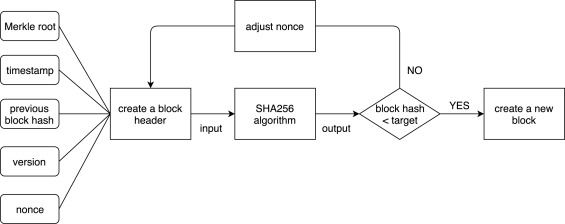
\includegraphics[width=4.5in, angle =0]{pow}
	\caption{Flow of PoW}
	\label{fig:pow}
\end{figure}

\textbf{PoS (Proof of Stake):} In PoS, selecting which node creates a new block
depends on the held take rather than the computational power. Node till need to solve
a SHA256 puzzle, but the nonce does not need to be adjusted, instead the key to solve
the puzzle is the amount of stake. Nxt and Ouroboros adopt PoS and Ethereum plans to
transition from PoW to PoS. This consensus protocol guarantees like
PoW eventual consistency. 

\begin{figure}[h]
	\centering
	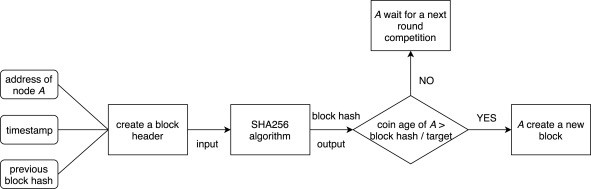
\includegraphics[width=4.5in, angle =0]{pos}
	\caption{Flow of PoS}
	\label{fig:pos}
\end{figure}


\textbf{DPoS (Delegated Proof of Stake):} The principle here is to let nodes who
hold stake to vote to elect block creators, this way delegating the job of creating
the blocks and reducing computational consumption. This is adopted by BitShares and EOS.

\begin{figure}[h]
	\centering
	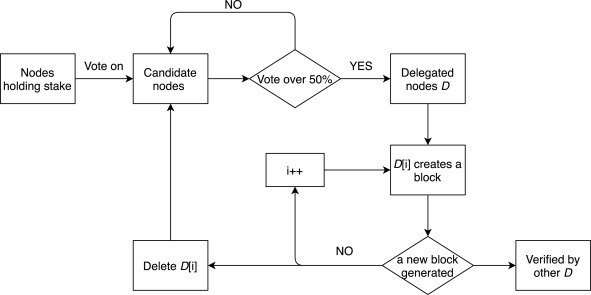
\includegraphics[width=4.5in, angle =0]{dpos}
	\caption{Flow of DPoS}
	\label{fig:dpos}
\end{figure}

\textbf{PBFT (Practical Byzantine Fault Tolerance):} PBFT is a Byzantine Fault 
Tolerance protocol with low algorithmic complexity, it contains five phases: request,
pre-prepare, prepare, commit and reply. PBFT guarantees nodes maintain a common state and take
a consistent action in each round, guarantees strong consistency and is adopted by
EOS to validate blocks while using DPoS for creation.

\begin{figure}[h]
	\centering
	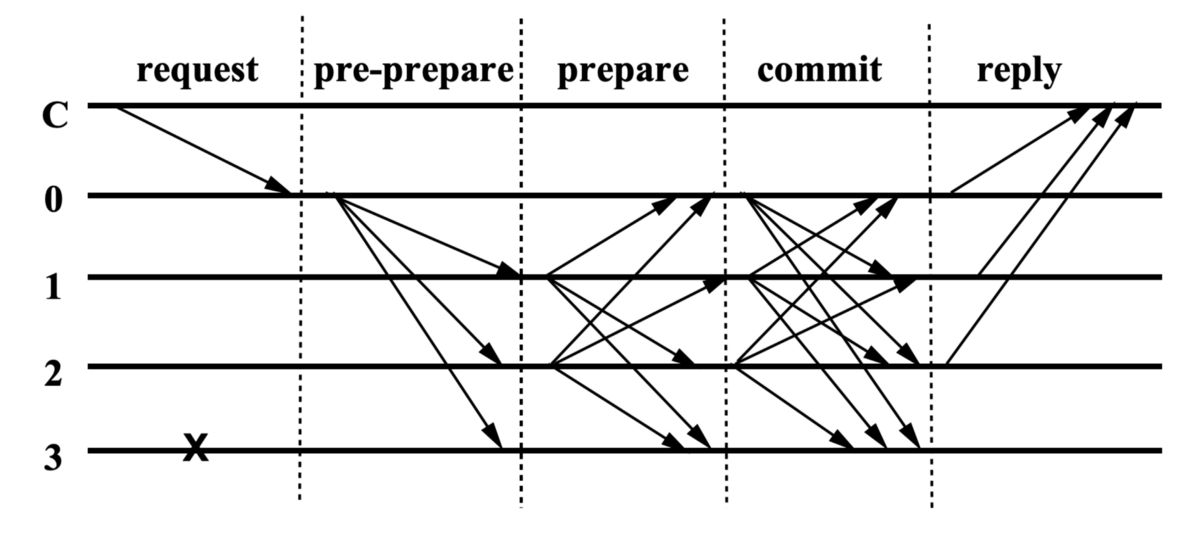
\includegraphics[width=4.5in, angle =0]{pbft}
	\caption{Flow of PBFT}
	\label{fig:pbft}
\end{figure}